\section{Auswertung}

\subsection{Induktion durch Änderung der Fläche und des Magnetfeldes}

Die Abbildungen \ref{plot:ui_by_omega} und \ref{plot:ui_by_i} zeigen die Aufgezeichnete induzierte Spannung in Abhängigkeit von der Drehfrequenz der Induktionsspule bzw. dem Strom durch die Helmholtz-Spule. Da wir die Drehfrequenz der Induktionsspule nicht exakt einstellen konnten, mussten wir diese durch die Frequenz der induzierten Wechselspannung ermitteln. Das Oszilloskop wies hierbei für niedrige Frequenzen hohe Schwankungen auf, weshalb der Fehler der niedrigeren Kreisfrequenzen in Abbildung \ref{plot:ui_by_omega} größer ist.

\begin{figure}[H]
    \centering
    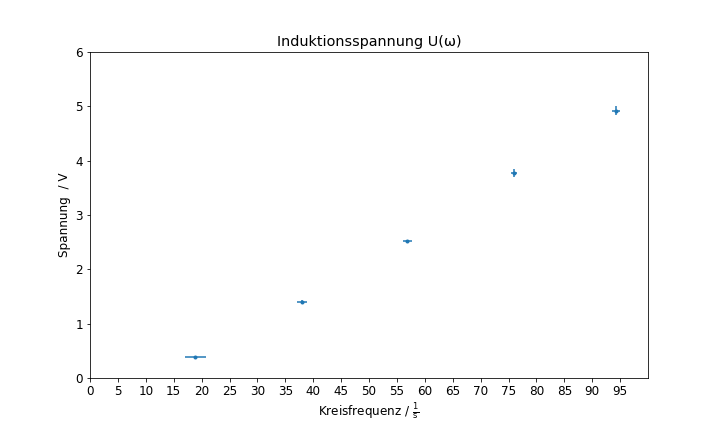
\includegraphics[width=0.8\textwidth]{files/ui_by_omega.png}
    \caption{Induzierte Spannung in Abhängigkeit von der Drehfrequenz der Induktionsspule}
    \label{plot:ui_by_omega}
\end{figure}

\begin{figure}[H]
    \centering
    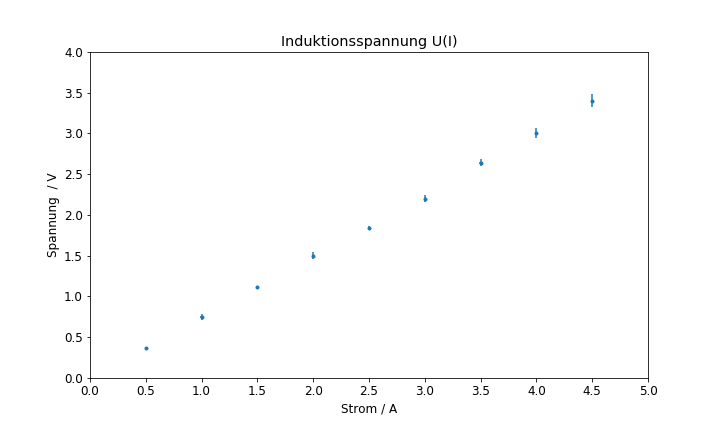
\includegraphics[width=0.8\textwidth]{files/ui_by_i.png}
    \caption{Induzierte Spannung in Abhängigkeit vom Strom durch die Helmholtz-Spule}
    \label{plot:ui_by_i}
\end{figure}

Wie auch von der mathematischen Beschreibung, dem Induktionsgesetz, vorhergesagt, weisen beide Szenarien ein lineares Verhältnis auf. Mithilfe einer linearen Regression können wir die Steigung dieses linearen Verhältnisses ermitteln, zu sehen in den Abbildungen \ref{plot:ui_by_omega_fit} und \ref{plot:ui_by_i_fit}.

\begin{figure}[H]
    \centering
    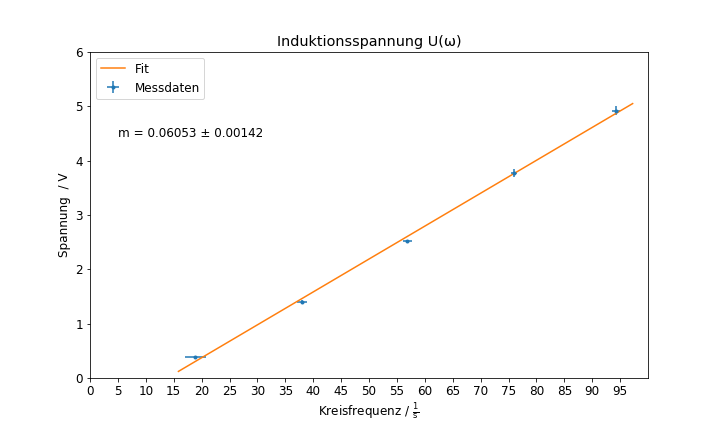
\includegraphics[width=0.8\textwidth]{files/ui_by_omega_fit.png}
    \caption{Induzierte Spannung in Abhängigkeit von der Drehfrequenz der Induktionsspule mit linearem Fit}
    \label{plot:ui_by_omega_fit}
\end{figure}

\begin{figure}[H]
    \centering
    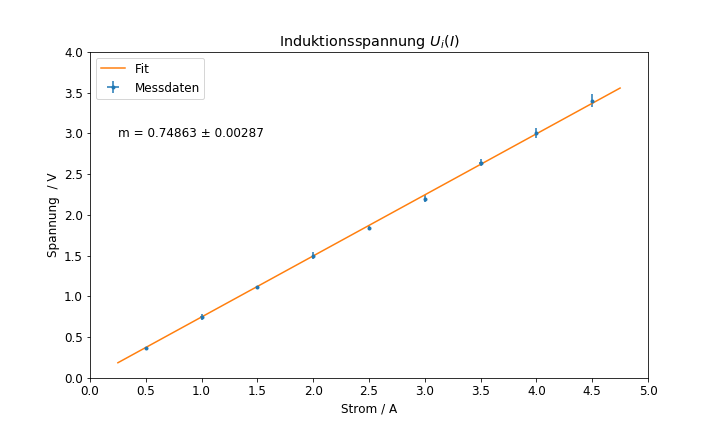
\includegraphics[width=0.8\textwidth]{files/ui_by_i_fit.png}
    \caption{Induzierte Spannung in Abhängigkeit vom Strom durch die Helmholtz-Spule mit linearem Fit}
    \label{plot:ui_by_i_fit}
\end{figure}

Wir betrachten nun genauer das Diagramm in Abbildung \ref{plot:ui_by_omega_fit}, also die Frequenzabhängigkeit der Induktionsspannung. Wir können in der Formel für die Spitzenspannung aus dem Einleitungsteil
\begin{align}
    U_{i,peak}(\omega) = B A N \omega
\end{align}
die Steigung der Gerade mit $m = BAN$ identifizieren. Stellen wir diese nach $B$ um, so erhalten wir mit $N = 4000$ und $A = 41.7 \cdot 10^{-4} \si{m^2}$ eine magnetische Flussdichte von
\begin{align}
    B_{exp} = \frac{m}{A N} \pm \frac{\Delta m}{A N} = (3.63 \pm 0.08) \cdot 10^{-3}\, \si{T}.
\end{align}

Die theoretische Vorhersage für die magnetische Flussdichte im Zentrum der Helmholtz-Spule, gegeben durch Gleichung \ref{eq:b_hh} entspricht
\begin{align}
    \qty|\va{B}(0)| = \frac{8}{\sqrt{125}} \frac{\mu_0 N (I \pm \Delta I)}{R} &= \frac{8}{\sqrt{125}} \frac{\mu_0 \cdot  124 \cdot (4.0 \pm \Delta 0.1)}{0.1475 \si{m^2}}\\[1em]
    &= (3.02 \pm 0.08) \cdot 10^{-3}\, \si{T}.
\end{align}

Aus den Werten erkennen wir, dass die experimentell verzeichnete magnetische Felddichte leicht höher ist, als die theoretisch vorhergesagte. Mögliche Ursachen für diesen Unterschied werden wir im letzten Kapitel diskutieren.

\subsection{Auswirkung des Winkels auf die Induktionsspannung}

Für die folgenden Versuchsteile wurde an die Helmholtz-Spule eine Wechselspannung der Kreisfrequenz $\Omega$ angelegt. Abbildung \ref{plot:ui_by_alpha} zeigt die induzierte Spannung aufgetragen über den Winkel der Induktionsspule in der Helmholtz-Spule.

\begin{figure}[H]
    \centering
    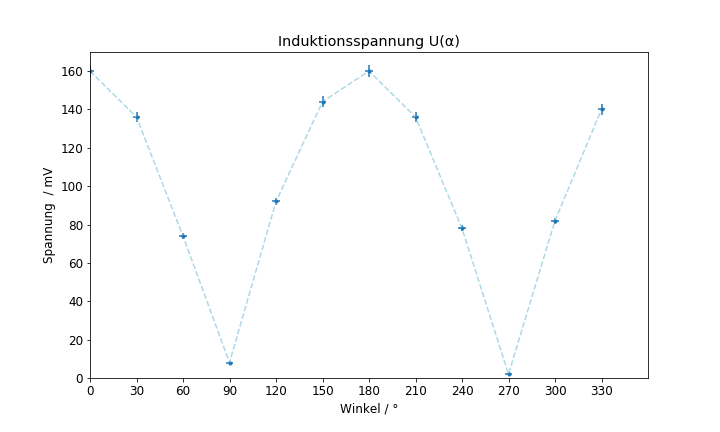
\includegraphics[width=0.8\textwidth]{files/ui_by_alpha.png}
    \caption{Induzierte Spannung in Abhängigkeit des Winkels der Induktionsspule}
    \label{plot:ui_by_alpha}
\end{figure}

Nach Gleichung \ref{eq:ui_ac_angle} weist die Induktionsspannung in diesem Fall eine Abhängigkeit der Form $U_I \sim \qty|\cos(\alpha)|$ auf. Dies deutet sich bereits in Abbildung \ref{plot:ui_by_alpha} und ist im Fit (Abbildung \ref{plot:ui_by_alpha_fit}) noch einmal deutlicher zu erkennen.

\begin{figure}[H]
    \centering
    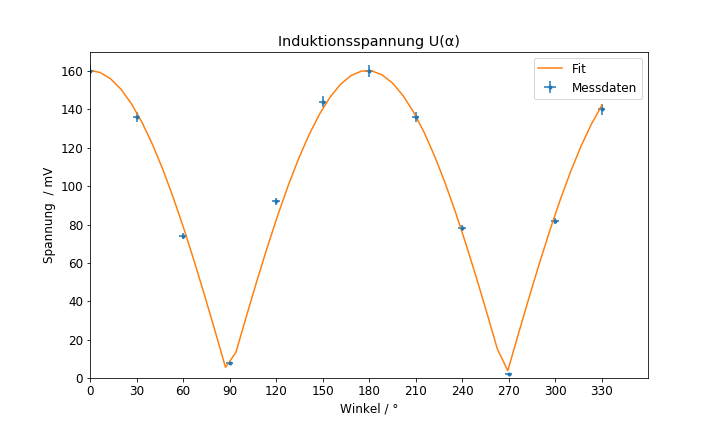
\includegraphics[width=0.8\textwidth]{files/ui_by_alpha_fit.png}
    \caption{Induzierte Spannung in Abhängigkeit des Winkels der Induktionsspule mit Fit}
    \label{plot:ui_by_alpha_fit}
\end{figure}

Für die nun folgenden Betrachtungen brachten wir die Induktionsspule wieder in eine horizontale Stellung in der Helmholtz-Spule.

\subsection{Verhältnis von induzierter und angelegter Spannung}

Abbildung (\ref{plot:ui_to_uhh_by_f}) zeigt das Verhältnis von induzierter zu angelegter Spannung $\frac{U_{\text{ind}}}{U_{\text{Hh}}}$ über der Kreisfrequenz $\Omega$ der angelegten Spannung.

\begin{figure}[H]
    \centering
    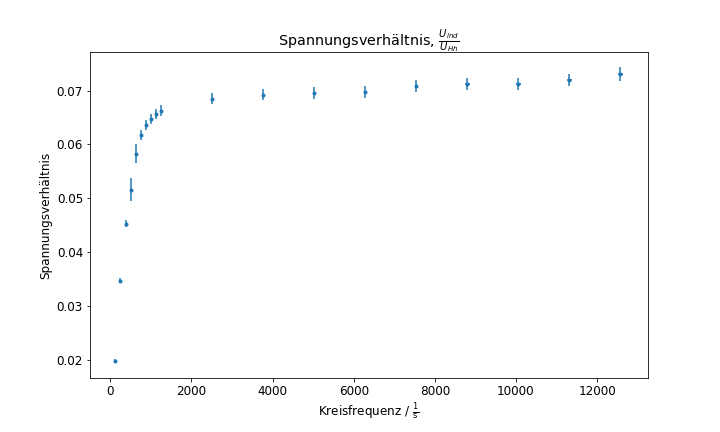
\includegraphics[width=0.8\textwidth]{files/ui_to_uhh_by_f.png}
    \caption{Verhältnis von induzierter und angelegter Spannung in Abhängigkeit von der Frequenz}
    \label{plot:ui_to_uhh_by_f}
\end{figure}

Es ist zu erkennen, dass sich das Verhältnis allmählich einer Asymptote bei ca. $0.07$ anschmiegt. Vergleichbar dazu zeigt Abbildung \abbref{plot:i_by_acf}, dass der Strom durch die Helmholtz-Spule mit zunehmender Frequenz der angelegten Wechselspannung abnimmt.

\begin{figure}[H]
    \centering
    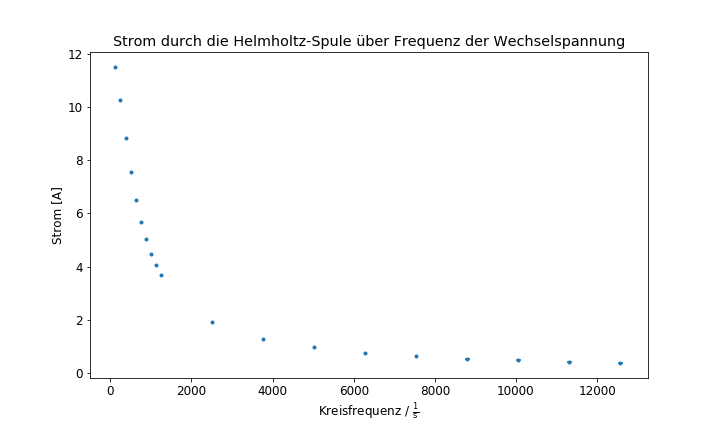
\includegraphics[width=0.8\textwidth]{files/i_by_acf.png}
    \caption{Strom durch die Helmholtz-Spule in Abhängigkeit von der Frequenz}
    \label{plot:i_by_acf}
\end{figure}

Diese Beobachtung ist durch die im Theorieteil erwähnte Selbstinduktion der Helmholtz-Spule zu erklären. Diese verursacht einen Strom, welcher gegen den angelegten Strom gerichtet ist. Um die Selbstinduktion noch einmal genauer zu untersuchen, betrachten wir in \abbref{plot:rhh_by_f} den Widerstand der Helmholtz-Spule, erneut abgetragen über der Frequenz der Wechselspannung.

\begin{figure}[H]
    \centering
    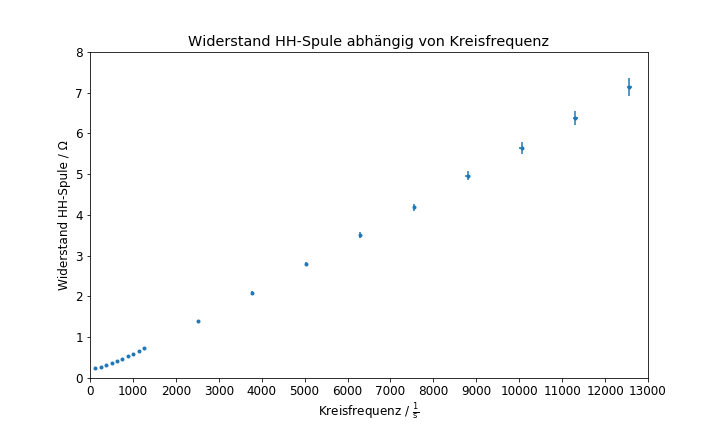
\includegraphics[width=0.8\textwidth]{files/rhh_by_f.png}
    \caption{Widerstand der Helmholtz-Spule in Abhängigkeit von der Frequenz}
    \label{plot:rhh_by_f}
\end{figure}

Der Widerstand zeigt einen nahezu linearen anstieg in Abhängigkeit von der Frequenz, durch welchen wir mittels linearer Regression eine Gerade legen können. Das Resultat des Fittings ist in \abbref{plot:rhh_by_f_fit} zu sehen.

\begin{figure}[H]
    \centering
    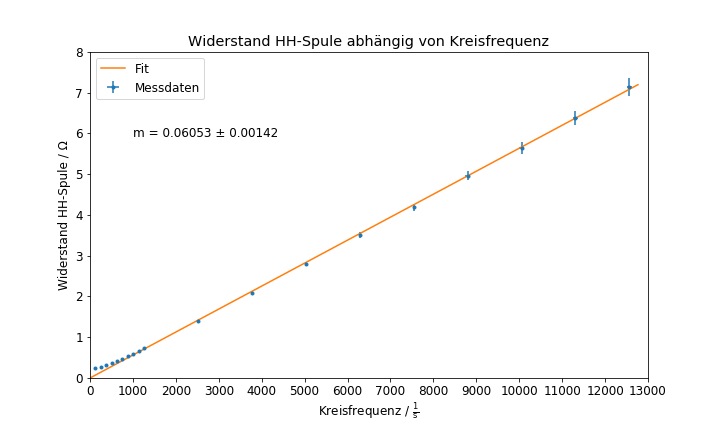
\includegraphics[width=0.8\textwidth]{files/rhh_by_f_fit.png}
    \caption{Widerstand der Helmholtz-Spule in Abhängigkeit von der Frequenz mit linearem Fit}
    \label{plot:rhh_by_f_fit}
\end{figure}

Wie in Gleichung \ref{eq:indukt_widerst} aufgezeigt, hängt der induktive Widerstand direkt von der Frequenz ab, wobei die Induktivität $L$ die Proportionalitätskonstante darstellt. Diese entspricht somit der Steigung der soeben gefitteten Gerade
\begin{align}
    m = L = (0.0605 \pm 0.0014)\, \si{H}.
\end{align}

\subsection{Untersuchung des Erdmagnetfeldes}

Um der Richtung der Feldlinien des Erdmagnetfeldes zu entsprechen, richteten wir die Induktionsspule zunächst mit einem Kompass in Nord-Süd-Richtung aus. Wir versetzen die Spule in eine Rotation der Kreisfrequenz $\omega = (14.8 \pm 0.2) \frac{2\pi}{\si{\second}}$. Die dabei gemessene induzierte Spannung betrug $U_i = (0.0740 \pm 0.0005) \si{V}$. Durch Umstellen der Formel für die Induktionsspannung
\begin{align}
    U_i = -BAN\omega
\end{align}
und einsetzen von Fläche und Windungszahl der Induktionsspule erhalten wir einen Wert von
\begin{align}
    B_{E,1} = (47.7 \pm 0.7)\unit{\micro\tesla}.
\end{align}

Dieses Resultat erhalten wir aus der Messung ohne Kompensation. Für die Messung mit Kompensation wurde mit der Helmholtz-Spule ein Magnetfeld erzeugt, welches die Vertikalkomponente des Erdmagnetfeldes kompensiert. Die beste Kompensation erhielten wir bei einem Strom von $I_{helm} = 0.0598 \pm 0.0002$\si{\ampere}. Nach Formel \ref{eq:b_hh} entspricht dies einer Vertikalkomponente von
\begin{align}
    B_{v} = (45.20 \pm 0.15)\si{\micro\tesla}.
\end{align}

Aus der verbleibenden Induktionsspannung von $U_i = (0.0225 \pm 0.0010) \unit{V}$ und einer Kreisfrequenz der Induktionsspule von $\omega = (14.7 \pm 0.3) \frac{2\pi}{\si{\second}}$ können wir, nach derselben Formel wie oben, eine horizontale Feldkomponente von
\begin{align}
    B_{h} = (14.6 \pm 2.3)\si{\micro\tesla}
\end{align}
berechnen.

Die beiden Feldkomponenten bilden zusammen mit der absoluten Magnetfelddichte aus dem ersten Teil ein rechtwinkliges Dreieck, wie auch in \ref{fig:erdmagnetfeld} aus dem Einleitungsteil zu sehen. Den Winkel der Hypotenuse dieses Dreiecks berechnen wir aus den beiden Komponenten mittels
\begin{align}
    \alpha = \arctan(\frac{B_{v}}{B_{h}}) = 72.10\si{\degree}.
\end{align}

Der Fehler des Winkels berechnet sich nach
\begin{gather}
    \Delta \alpha = \sqrt{\qty(\frac{B_{h} \cdot \Delta B_{v}}{B_{v}^2 + B_{h}^2})^2 + \qty(\frac{B_{v} \cdot \Delta B_{h}}{B_{v}^2 + B_{h}^2})^2}
    \intertext{zu}
    \Delta \alpha = 2.68\si{\degree}.
\end{gather}

% literatur 65° 15' = 65.25° -> 2.56 * sigma (2.68)